%%    TEMPLATE for articles submitted to SPMS proceedings 2012
%%
%%
%%     Please do not remove lines commented out with %+
%%           these are for the editors' use.
%%
% !!!!!!!!!!!!!!!!!!!!!!!!!!!!!!!!!!!!!!!!!!!!!!!!!!!!!!!!!!!!!!!!!!!!!!!
% !!!!!!!!!!!   Don't modify template to \begin{document}     !!!!!!!!!!!
% !!!!!!!!!!!!!!!!!!!!!!!!!!!!!!!!!!!!!!!!!!!!!!!!!!!!!!!!!!!!!!!!!!!!!!!


\documentclass[a4paper,12pt,twoside]{article}
\usepackage{epsfig}
\usepackage{amsfonts}
\usepackage{amsmath}
\usepackage{amssymb}
\usepackage{fancyheadings}
%\usepackage{fancyhdr}
\usepackage{theorem}
\usepackage{makeidx,showidx}
\usepackage{index}
\usepackage{multind}
\usepackage{longtable}
\usepackage{subfigure}


\input SPMSdefinitions


\begin{document}

\myhead

\thispagestyle{plain}
\titlehead


% !!!!!!!!!!!!!!!!!!!!!!!!!!!!!!!!!!!!!!!!!!!!!!!!!!!!!!!!!!!!!!!!!!!!!!!
% !!!                   START HERE                                   !!!
% !!!!!!!!!!!!!!!!!!!!!!!!!!!!!!!!!!!!!!!!!!!!!!!!!!!!!!!!!!!!!!!!!!!!!!!

\Title{Testing of robustness and efficiency of R\'{e}nyi divergence estimators of probability densities}

\titleshort{R\'{e}nyi divergence estimators}

\Author{Jan Ku\v{c}era, V\'{a}clav K\r{u}s}
\authorshort{J. Ku\v{c}era, V. K\r{u}s}
%+ \index{Regiano, D.}%
%+ \addcontentsline{toc}{part}{\titleall\\*\textit{\authors}}

\Institution{Department of Mathematics,
Faculty of Nuclear Sciences and Physical Engineering,
Czech Technical University in Prague,
Trojanova 13, 12000 Prague, Czech Republic}

\Email{kucerj28@fjfi.cvut.cz, vaclav.kus@fjfi.cvut.cz}


\Abstract{ In this contribution we study R\'{e}nyi pseudo-distance estimators which are based on minimization of information-theoretic divergences between empirical and hypothetical probability distribution. These distances are more robust (than e.g. MLE estimators) against outliers and other measurement errors potentially present in the data sets. Robustness of these estimators is described by influence function. In \cite{Vajda2009} and \cite{Demut2010} authors found explicit formulas for enumeration of R\'{e}nyi pseudodistances in normal families and for their influence functions. We focus on finding explicit formulas for other families (Weibull, Cauchy, Exponential) and finding influence functions for these estimators.
We perform computer simulations for pseudorandom contaminated and uncontaminated data sets, different sample sizes and different R\'{e}nyi pseudodistance parameters. }

\Keywords{R\'{e}nyi pseudodistances; $\phi-$divergences; robustness; minimum pseudodistance estimators}

{\normalsize


\section{Introduction and basic definitions}
In this contribution we study R\'{e}nyi pseudo-distance estimators which are based on the minimization of information-theoretic divergences between empirical and hypothetical probability distribution. They are not classical distances, because the symmetry or triangle inequality does not have to hold. Let $\mathcal{P} = \lbrace P_\theta : \theta \in \Theta \subset \mathbb{R}^m \rbrace$ be a set of probability measures on measurable space $\left(\mathcal{X},\mathcal{A}\right)$.
We will apply the estimators in the statistical model with i.i.d. observations $X_1,\ldots,X_n$ governed by distribution $P_r$.
Since we are interested in robustness, we allow the case $P_r \notin \mathcal{P}$ and therefore we define another set $\mathcal{P}^+ = \mathcal{P} \cup \lbrace P_r \rbrace $. In this paper we take into consideration the distribution $P_r$ of contaminated data modeled as a mixture of distributions $P_r = (1-\varepsilon)P + \varepsilon Q$, where $\varepsilon$ is the the contamination level, $P$ is the distribution of the non-contaminated part of the data and $Q$ is the distribution of the contamination.

\begin{definition}
	We say that the mapping $\mathfrak{D}:\mathcal{P}\times\mathcal{P}^+ \rightarrow \mathbb{R}$ is a pseudo-distance between probability measures $P \in \mathcal{P}$ and $Q \in \mathcal{P}^+$ if it holds		
		\begin{equation}
			\mathfrak{D}(P_\theta,Q) \geq 0 \quad \textit{for all } \theta \in \Theta \quad \text{and} \quad Q \in \mathcal{P}^+
		\end{equation}
		and 		
		\begin{equation}
			\mathfrak{D}(P_\theta,P_{\tilde{\theta}})=0 \; \Leftrightarrow \; \theta=\tilde{\theta}.
		\end{equation}	
	This pseudo-distance is decomposable if there exist functionals such that
		 $\mathfrak{D}^0:\mathcal{P}\rightarrow\mathbb{R}$, $ \mathfrak{D}^1:\mathcal{P}^+ \rightarrow \mathbb{R}$ and measurable mapping
		  $\rho_\theta : \mathcal{X} \rightarrow \mathbb{R}$, $ \theta \in \Theta$, so that for all $\theta \in \Theta$ and for all $Q \in \mathcal{P}^+$ the expectation $\int{\rho_\theta }\mathrm{d}Q$ exists and
		\begin{equation}
			\mathfrak{D} (P_\theta, Q) = \mathfrak{D}^0 (P_\theta) + \mathfrak{D}^1 (Q) + \int \rho_\theta \mathrm{d}Q.
		\end{equation}
\end{definition}

\begin{definition}
	We say that a functional $T_\mathfrak{D}:\mathcal{Q} \rightarrow \Theta$, for $\mathcal{Q}=\mathcal{P}^+ \cup \mathcal{P}_{\text{emp}}$	defines minimum pseudo-distance estimator (min $\mathfrak{D}$-estimator) if $\mathfrak{D}(P_\theta,Q)$ is a decomposable pseudo-distance on $\mathcal{P}\times\mathcal{P}^+$ and parameters $T_\mathfrak{D}(Q) \in \Theta$ minimize $\mathfrak{D}^0 + \int{\rho_\theta}\mathrm{d}Q$, that means
	\begin{equation}
		T_\mathfrak{D}(Q) = \arg\min_{\theta \in \Theta} \left[ \mathfrak{D}^0(P_\theta) + \int{\rho_\theta}\mathrm{d}Q \right] \quad \forall Q \in \mathcal{Q}.
	\end{equation}
\end{definition}
In particular, for $Q = P_n = \frac{1}{n}\sum_{i-1}^n \delta_{X_i} \in \mathcal{P}_{emp}$
\begin{equation}
	\hat{\theta}_{\mathfrak{D},n} =T_\mathfrak{D}(P_n)  = \arg\min_{\theta \in \Theta}\left[ \mathfrak{D}^0(P_\theta) + \dfrac{1}{n} \sum_{i-1}^n \rho_\theta (X_i) \right].
\end{equation}
Every min $\mathfrak{D}$-estimator is Fisher consistent in the sense that
\begin{equation}
	T_\mathfrak{D}(P_{\theta_0}) = \arg\min_{\theta \in \Theta} \mathfrak{D}(P_\theta, P_{\theta_0}) = \theta_0,\quad \forall \theta_0 \in \Theta.
\end{equation}

\begin{theorem}
Let for some $\beta>0$ it holds that
	\begin{equation*}
			p^\beta, q^\beta,\ln{p} \in \mathrm{L}_1(Q), \quad \forall P \in \mathcal{P}, Q \in \mathcal{P^+}.
	\end{equation*}
	Then for all $\alpha$, $0 < \alpha \leq \beta$, and for $P \in \mathcal{P}, \; Q \in \mathcal{P^+} $ the expression
	\begin{equation}
		\mathfrak{R}_\alpha (P,Q) = \dfrac{1}{1+\alpha}\ln{\left( \int{p^\alpha \mathrm{d}P } \right)} +
		\dfrac{1}{\alpha (1+\alpha)}\ln{\left( \int{q^\alpha \mathrm{d}Q } \right)} -
		\dfrac{1}{\alpha} \ln{\left( \int{p^\alpha \mathrm{d}Q } \right)}
	\end{equation}
		represents the family of pseudo-distances decomposable in the sense of
	\begin{equation*}
		\mathfrak{R}_\alpha (P,Q) = \mathfrak{R}_\alpha^0 (P) + \mathfrak{R}_\alpha^1 (Q) - \dfrac{1}{\alpha} \ln{\left( \int{p^\alpha \mathrm{d}Q } \right)},
	\end{equation*}	
	where
	\begin{equation*}
		\mathfrak{R}_\alpha^0 (P) = \dfrac{1}{1+\alpha}\ln{\left( \int{p^\alpha \mathrm{d}P } \right)}, \quad \mathfrak{R}_\alpha^1 (Q) = \dfrac{1}{\alpha (1+\alpha)}\ln{\left( \int{q^\alpha \mathrm{d}Q } \right)}.
	\end{equation*}
	Moreover, for $\alpha \searrow 0$ it holds
	\begin{equation*}
		\mathfrak{R}_0 (P,Q) = \lim_{\alpha \searrow 0} \mathfrak{R}_\alpha (P,Q) =  \int{\left( \ln{q} - \ln{p} \right)\mathrm{d}Q}.
	\end{equation*}
\end{theorem}

\noindent The R\'{e}nyi pseudo-distance estimator is then determined by

\begin{equation}
	T_{\mathfrak{R}_\alpha}(Q) =
	\begin{cases}
		 \arg \min_{\theta} \left[\frac{1}{1+\alpha} \ln(\int p_\theta^\alpha\mathrm{d}P_\theta) - \frac{1}{\alpha} \ln(\int p_\theta^\alpha\mathrm{d}Q) \right] & \text{for } 0 < \alpha \leq \beta, \\
		 \arg \min_{\theta} \left[- \ln(\int p_\theta\mathrm{d}Q) \right] & \text{for } \alpha = 0.
	\end{cases}	
\end{equation}

We are interested in the estimators, where we replace the hypothetical distribution $P_r$ with the empirical distribution $P_n$. It means that the family of minimum R\'{e}nyi pseudo-distance estimators defined as $\theta_{n,\alpha} = T_{\mathfrak{R}_\alpha}(P_n)$ for $T_{\mathfrak{R}_\alpha}(Q) \in \Theta$ with $Q \in \mathcal{P}^+$ satisfies the condition

\begin{equation}
	\theta_{\alpha,n} =
	\begin{cases}
		\displaystyle{ \arg \max_{\theta \in \Theta} C_\alpha\left( \theta \right)^{-1} \frac{1}{n} \sum_{i=1}^n p_{\theta}^{\alpha}\left( X_i \right) } & \text{for } 0 < \alpha \leq \beta, \\
		\displaystyle{ \arg \max_{\theta \in \Theta}  \frac{1}{n} \sum_{i=1}^n \ln p_{\theta}\left( X_i \right) } & \text{for } \alpha = 0.
	\end{cases}	
	\label{JK-Renyi-estimator_formula}
\end{equation}
In \cite{Vajda2009}, the influence function for R\'{e}nyi divergence estimators is derived as
\begin{equation}
\mathrm{IF}(x;T_{\mathfrak{R}_\alpha},\theta) = -\mathbf{I}^{-1}_{\alpha}(\theta) \left[ p_\theta^\alpha(x) (s_\theta (x) - c_\alpha (x)) \right], \label{JK-IF}
\end{equation}
where
\begin{center}
\begin{tabular}{r l}
$s_\theta = \dfrac{\mathrm{d}}{\mathrm{d}\theta} \ln p_\theta, \quad$ & $ \dot{s}_\theta = \left( \dfrac{\mathrm{d}}{\mathrm{d}\theta} \right)^T s_\theta,$ \\
$c_\alpha(\theta) = \dfrac{\int p_\theta^{1+\alpha}s_\theta \mathrm{d}\lambda}{\int p_\theta^{1+\alpha} \mathrm{d}\lambda}, \quad$ & $\dot{c}_\alpha(\theta)= \left( \dfrac{\mathrm{d}}{\mathrm{d}\theta} \right)^T c_\alpha(\theta),$  \\
\end{tabular}
\end{center}
and
\begin{equation}
\mathbf{I}_{\alpha}(\theta) = \int{ \left[\dot{s}_\theta - \dot{c}_\alpha(\theta) - \alpha(s_\theta - c_\alpha(\theta))(c^T_\alpha(\theta) - s^T_\theta) \right] p_\theta^{1+\alpha} \mathrm{d}\lambda}.
\end{equation}
%
We use these influence functions to demonstrate the robustness of minimum R\'{e}nyi pseudodistance estimator. There are more important characteristics, but we will be interested in two of them. First one is the \textit{gross-error sensitivity} characterized by $\gamma^* = \sup_x |\mathrm{IF}(x;T_{\mathfrak{R}_\alpha},\theta)|$. We require it to be finite, in other words, we want the influence function to be bounded. The other one is called \textit{rejection point} and is defined as
$\rho^* = \inf\lbrace  r > 0 \; | \; \mathrm{IF}(x;T_{\mathfrak{R}_\alpha},\theta) = 0 \; \mathrm{for} \; |x|> r \rbrace$. It describes the values of samples, which will be treated as outliers and finally rejected.

\section{Application to specific families}

In \cite{Vajda2009} the authors present formulas for computing and evaluating R\'{e}nyi pseudodistance estimator in normal family. Our goal was to study these estimators in other families. In the next chapter we present our results together with some examples.

%%%%%%%%%%%%%%%%%%%%%%%%%%%%%%%%%%%%%%%% LAPLACE %%%%%%%%%%%%%%%%%%%%%%%%%%%%%%%%%%%%%%%%%%%%

\subsection*{Laplace family}
We use the minimum R\'{e}nyi estimators for parameter $\theta = (\mu,\lambda)$ in Laplace family, where the probability density is
\begin{equation}
	p_\theta = \frac{1}{2\lambda} e^{-\frac{|x-\mu|}{\lambda}}, \qquad \mu\in \mathbb{R}, \lambda>0,
\end{equation}
and therefore the estimator according to \eqref{JK-Renyi-estimator_formula} is
\begin{equation}
	\theta_{\alpha,n} = \arg \max_{\theta \in \Theta} \left[ (2\lambda)^{-\frac{\alpha}{1+\alpha}} \frac{1}{n} \sum_{i=1}^n \exp \left[-\alpha\frac{|x_i-\mu|}{\lambda} \right] \right].
\end{equation}
% tabulka a obrazek eref %%%%%%

\begin{table}[htb] \footnotesize
\begin{center}
\begin{tabular}{ccc}
	\begin{tabular}{|c|ccc|}
	\hline
	$\alpha\backslash n$ &&  $500$ & \\
	\hline
	& $m(\mu)$ & $s(\mu)$ & $eref(\mu)$ \\
	& $m(\lambda)$ & $s(\lambda)$ & $eref(\lambda)$ \\
	\hline
	$0.0$ & $ -0.005 $ & $ 0.071 $ & $ 1.000 $\\
	 & $ 4.593 $ & $ 3.617 $ & $ 1.000 $\\
	\hline
	$0.05$ & $ -0.000 $ & $ 0.071 $ & $ 1.018 $\\
	 & $ 4.168 $ & $ 3.192 $ & $ 1.284 $\\
	\hline
	$0.1$ & $ 0.003 $ & $ 0.066 $ & $ 1.163 $\\
	 & $ 3.719 $ & $ 2.741 $ & $ 1.742 $\\
	\hline
	$0.2$ & $ -0.002 $ & $ 0.068 $ & $ 1.098 $\\
	 & $ 2.888 $ & $ 1.914 $ & $ 3.570 $\\
	\hline
	$0.3$ & $ -0.004 $ & $ 0.068 $ & $ 1.108 $\\
	 & $ 2.215 $ & $ 1.241 $ & $ 8.490 $\\
	\hline
	$0.5$ & $ 0.001 $ & $ 0.069 $ & $ 1.056 $\\
	 & $ 1.546 $ & $ 0.568 $ & $ 40.516 $\\
	\hline
	$1.0$ & $ 0.003 $ & $ 0.074 $ & $ 0.927 $\\
	 & $ 1.221 $ & $ 0.256 $ & $ 199.663 $\\
	\hline
	\end{tabular}
&&
	\begin{tabular}{c}
		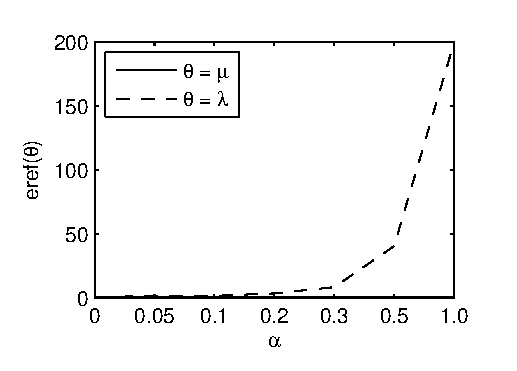
\epsfig{file=Laplace-e04-eref.eps, height=2.5in}
	\end{tabular}
\\
\end{tabular}
\end{center}
\caption{R\'{e}nyi estimates: $p_\theta = \mathrm{L}(0,1)$, contamination: $(1-\varepsilon)\mathrm{L}(0,1) + \varepsilon \mathrm{L}(0,10)$, $\varepsilon =  0.4$}
\label{tabJK:laplace-eref}
\end{table}

\noindent To obtain Table \ref{tabJK:laplace-eref} we generated contaminated data (number of observations $n = 500$) as a mixture of two Laplace distributions $(1-\varepsilon)\mathrm{L}(0,1) + \varepsilon \mathrm{L}(0,10)$ with $\varepsilon =  0.4$.
Then we used R\'{e}nyi estimators and estimated the parameters $\mu$, $\lambda$, consequently we repeated this process $m = 1000$ times. The numbers in the table represent mean value and variance of the estimated parameters. In the last column, the relative efficiency is stated and is given by
\begin{equation}
eref(p) = \sqrt{\dfrac{\frac{1}{m}\sum_{k=1}^m (\hat{p}_{\mathrm{MLE} ,k} - p_{\mathrm{real}})^2}{\frac{1}{m}\sum_{k=1}^m (\hat{p}_{\alpha,k} - p_{\mathrm{real}})^2}},
\end{equation}
where $ \hat{p}_{\mathrm{MLE},k}$ is the maximum likelihood MLE estimator, $p_{\mathrm{real}}$ is the real parameter of the contaminated distribution and $\hat{p}_{\alpha,k}$ is the minimal R\'{e}nyi estimator. As we can see, the efficiency improves with increasing $\alpha$. This depends on the level of contamination, estimators with higher $\alpha$ are more robust against outliers, so with increasing level of contamination with more dispersed observations the relative efficiency will grow up, because of the robustness against outliers.

%%%%%%%%%%%%%%%%%%%%%%%%%%%%%%%%% laplace - IF %%%%%%%%%%%%%%%%%%%%%%%%%%%%%%%%%%%%%%%
If we compute the influence functions according to \eqref{JK-IF}, where we put $\theta = \mu$ (estimated parameter), $ \lambda := 1$ (known parameter), respectively $\theta = \lambda$, $ \mu := 0$, we get
\begin{equation}
	\mathrm{IF}(x;T_{\mathfrak{R}_\alpha},\mu) = (1+\alpha )^{\frac{3}{2}} (x-\mu )  e^{-\frac{\alpha}{2} (x-\mu )^2}, % IF(x,mu)
	\label{JK-IF-laplace-mu}
\end{equation}
respectively
\begin{equation}
	\mathrm{IF}(x;T_{\mathfrak{R}_\alpha},\lambda) = (1 + \alpha)^2 \left(-\lambda + (1 + \alpha)|x|\right)  e^{-\frac{\alpha|x|}{\lambda}}	.
% IF(x,sigma)
	\label{JK-IF-laplace-lambda}
\end{equation}
\begin{figure}[htb]
\begin{center}
\begin{tabular}{c c }
	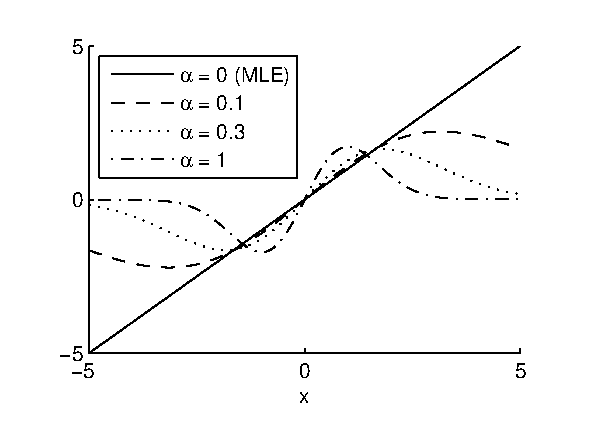
\epsfig{file=Laplace-IF-mu.eps, height=2.1in}
	&
	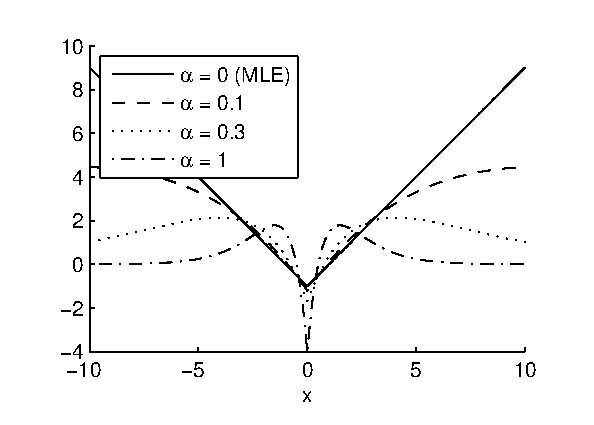
\epsfig{file=Laplace-IF-lambda.eps, height=2.1in}
	\\
	$\mathrm{IF}(x;T_{\mathfrak{R}_\alpha},\mu = 0) $, $\lambda = 1$ is known
	&
	$\mathrm{IF}(x;T_{\mathfrak{R}_\alpha},\lambda = 1)$, $\mu = 0$ is known
	\\
\end{tabular}
\caption{Influence functions of R\'{e}nyi estimator for Laplace distribution.}
\end{center}
\label{figJK:laplace-if}
\end{figure}
We can see from \eqref{JK-IF-laplace-mu} and \eqref{JK-IF-laplace-lambda} that our estimators are robust for $\alpha > 0$ in the sense that their influence functions are bounded. Also with higher $\alpha$ they are robust against outliers since $\lim_{x\rightarrow \pm\infty}\mathrm{IF}(x;T_{\mathfrak{R}_\alpha},\cdot) = 0 $. Moreover, the convergence is faster with increasing $\alpha$ due to the term $e^{-\alpha x}$ vanishing in both functions.

%%%%%%%%%%%%%%%%%%%%%%%%%%%%%%%%%%%%%%%% Exponential %%%%%%%%%%%%%%%%%%%%%%%%%%%%%%%%%

\subsection*{Exponential family}
If we use min R\'{e}nyi estimators in the exponential family, due to similarity with the Laplace family, we get very similar results. We have probability density
\begin{equation}
	p_\theta = \frac{1}{\lambda} e^{-\frac{x-\mu}{\lambda}}, \qquad \mu\in \mathbb{R}, \lambda>0,
\end{equation}
and therefore the estimator is
\begin{equation}
	\theta_{\mathfrak{R}_\alpha,n} = \arg \max_{\theta \in \Theta} \lambda^{-\frac{\alpha}{1+\alpha}} \frac{1}{n}\sum_{i=1}^n \exp \left[-\alpha\frac{x_i-\mu}{\lambda} \right].
\end{equation}

\begin{table}[htb] \footnotesize
\begin{center}
\begin{tabular}{ccc}
	\begin{tabular}{|c|ccc|}
	\hline
	$\alpha\backslash n$ && $500$ & \\
	\hline
	& $m(\mu)$ & $s(\mu)$ & $eref(\mu)$ \\
	& $m(\lambda)$ & $s(\lambda)$ & $eref(\lambda)$ \\
	\hline
	$0.0$ & $ 0.003 $ & $ 0.004 $ & $ 1.000 $\\
	 & $ 4.659 $ & $ 3.683 $ & $ 1.000 $\\
	\hline
	$0.05$ & $ 0.003 $ & $ 0.005 $ & $ 0.951 $\\
	 & $ 4.184 $ & $ 3.207 $ & $ 1.319 $\\
	\hline
	$0.1$ & $ 0.003 $ & $ 0.004 $ & $ 1.070 $\\
	 & $ 3.738 $ & $ 2.761 $ & $ 1.780 $\\
	\hline
	$0.2$ & $ 0.003 $ & $ 0.005 $ & $ 0.932 $\\
	 & $ 2.887 $ & $ 1.911 $ & $ 3.712 $\\
	\hline
	$0.3$ & $ 0.003 $ & $ 0.004 $ & $ 1.005 $\\
	 & $ 2.196 $ & $ 1.224 $ & $ 9.057 $\\
	\hline
	$0.5$ & $ 0.003 $ & $ 0.005 $ & $ 0.738 $\\
	 & $ 1.545 $ & $ 0.569 $ & $ 41.931 $\\
	\hline
	$1.0$ & $ 0.007 $ & $ 0.012 $ & $ 0.145 $\\
	 & $ 1.217 $ & $ 0.255 $ & $ 208.991 $\\
	\hline
	\end{tabular}
&&
	\begin{tabular}{c}
		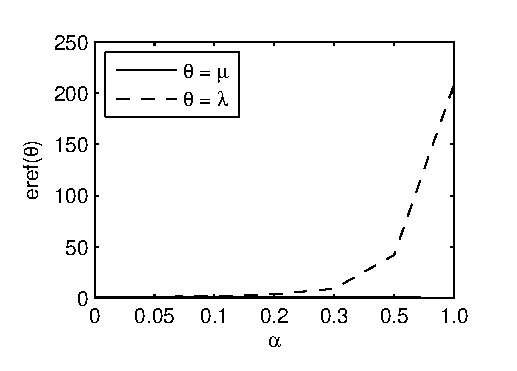
\epsfig{file=Exp-e04-eref.eps, height=2.5in}
	\end{tabular}
\\
\end{tabular}
\end{center}
\caption{R\'{e}nyi estimates: $p_\theta = \mathrm{E}(0,1)$, contamination: $(1-\varepsilon)\mathrm{E}(0,1) + \varepsilon \mathrm{E}(0,10)$, $\varepsilon =  0.4$.}
\label{tabJK:exponential-eref}
\end{table}

\noindent Table \ref{tabJK:exponential-eref} was generated in the same manner as Table \ref{tabJK:laplace-eref}, but in this case we used mixture of two exponential distributions with different parameters. Relative efficiency of estimators of $\lambda$ are very similar to the estimators in Laplace family, but in this case the efficiency of estimators of $\mu$ is decreasing with higher $\alpha$. Although the efficiency is low, we can see that the estimates are really close to the true value for all cases of $\alpha$. Here we can clearly see, that there has to be some experiments regarding the choice of $\alpha$ for the specific problem, because in this case it would be better to use $\alpha \sim 0.3$.

%%%%%%%%%%%%%%%%%%%% exp - IF %%%%%%%%%%%%%%%%%%%%%%%%%

We compute the influence functions according to \eqref{JK-IF}. When we put $\theta = \mu$, $ \lambda := 1$, for $\mathrm{IF}(x;T_{\mathfrak{R}_\alpha},\mu)$ we get the same result as in \eqref{JK-IF-laplace-mu}. For $\theta = \lambda $, $ \mu := 0$, we get
\begin{equation}
	\mathrm{IF}(x;T_{\mathfrak{R}_\alpha},\lambda) =	(1+\alpha )^2 ( - \lambda +(1+ \alpha)x) e^{-\frac{\alpha x}{\lambda }} % IF(x,lambda),
	\label{JK-IF-exponential-lambda}
\end{equation}
which differs from \eqref{JK-IF-laplace-lambda} only in the replacement of $x$ instead of $\vert x \vert$.
\begin{figure}[htb]
\begin{center}
\begin{tabular}{c c}
	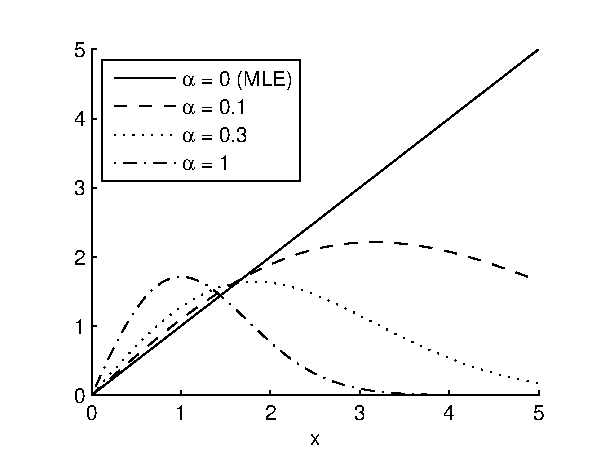
\epsfig{file=Exp-IF-mu.eps, height=2.1in}
	&
	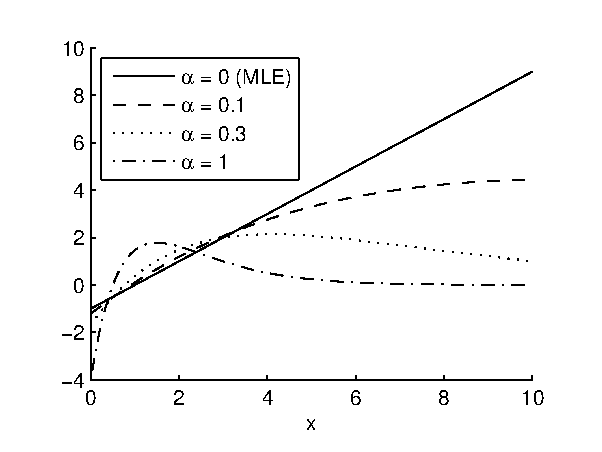
\epsfig{file=Exp-IF-lambda.eps, height=2.1in}
	\\
	$\mathrm{IF}(x;T_{\mathfrak{R}_\alpha},\mu = 0) $, $\lambda = 1$ is known
	&
	$\mathrm{IF}(x;T_{\mathfrak{R}_\alpha},\lambda = 1)$, $\mu = 0$ is known
	\\
\end{tabular}
\caption{Influence functions of R\'{e}nyi estimator for exponential distribution.}
\end{center}
\label{figJK:exponential-if}
\end{figure}

\noindent From \eqref{JK-IF-exponential-lambda} and Figure \ref{figJK:exponential-if} we can see, that the influence function has the same properties with respect to robustness as the influence function within the Laplace family.

%%%%%%%%%%%%%%%%%%%%%%%%%%%%%%%%%%%%%%%% Cauchy %%%%%%%%%%%%%%%%%%%%%%%%%%%%%%%%%%%%%%%%%%%%

\subsection*{Cauchy family}
For Cauchy family with parameters $\theta = (\mu,\sigma)$ and probability density
\begin{equation}
	p_\theta = \frac{1}{\pi\sigma} \left( 1 + \left( \frac{x-\mu}{\sigma} \right)^2 \right)^{-1}, \qquad \mu\in \mathbb{R}, \sigma>0,
\end{equation}
the minimal R\'{e}nyi pseudodistance estimator is given by
\begin{equation}
	\theta_{\alpha,n} = \arg \max_{\theta \in \Theta} \left[ \sigma^{-\frac{\alpha}{1+\alpha}} \frac{1}{n} \sum_{i=1}^n \left( 1 + \left( \frac{x_i-\mu}{\sigma} \right)^2 \right)^{-\alpha} \right].
\end{equation}

\begin{table}[htb] \footnotesize
\begin{center}
\begin{tabular}{ccc}
	\begin{tabular}{|c|ccc|}
	\hline
	$\alpha\backslash n$ && $500$ & \\
	\hline
	& $m(\mu)$ & $s(\mu)$ & $eref(\mu)$ \\
	& $m(\sigma)$ & $s(\sigma)$ & $eref(\sigma)$ \\
	\hline
	$0.0$ & $ 0.012 $ & $ 0.112 $ & $ 1.000 $\\
	 & $ 2.359 $ & $ 1.389 $ & $ 1.000 $\\
	\hline
	$0.05$ & $ -0.001 $ & $ 0.099 $ & $ 1.286 $\\
	 & $ 2.262 $ & $ 1.282 $ & $ 1.174 $\\
	\hline
	$0.1$ & $ -0.001 $ & $ 0.096 $ & $ 1.361 $\\
	 & $ 2.134 $ & $ 1.156 $ & $ 1.445 $\\
	\hline
	$0.2$ & $ 0.001 $ & $ 0.096 $ & $ 1.374 $\\
	 & $ 1.904 $ & $ 0.926 $ & $ 2.251 $\\
	\hline
	$0.3$ & $ -0.004 $ & $ 0.093 $ & $ 1.467 $\\
	 & $ 1.738 $ & $ 0.760 $ & $ 3.346 $\\
	\hline
	$0.5$ & $ -0.002 $ & $ 0.088 $ & $ 1.639 $\\
	 & $ 1.491 $ & $ 0.519 $ & $ 7.168 $\\
	\hline
	$1.0$ & $ -0.001 $ & $ 0.096 $ & $ 1.377 $\\
	 & $ 1.225 $ & $ 0.272 $ & $ 26.129 $\\
	\hline
	\end{tabular}
&&
	\begin{tabular}{c}
		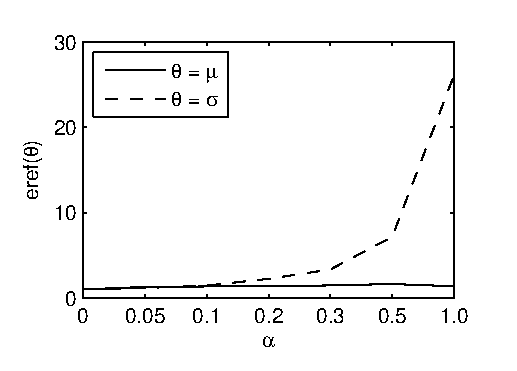
\epsfig{file=Cauchy-e04-eref.eps, height=2.5in}
	\end{tabular}
\\
\end{tabular}
\end{center}
\caption{R\'{e}nyi: $p_\theta = \mathrm{C}(0,1)$, data: $(1-\varepsilon)\mathrm{C}(0,1) + \varepsilon \mathrm{C}(0,10)$, $\varepsilon =  0.4$}
\label{tabJK:cauchy-eref}
\end{table}

\noindent In Table \ref{tabJK:cauchy-eref} we can see, that relative efficiency of R\'{e}nyi estimators increases with higher $\alpha$ in estimates of both parameters.


%%%%%%%%%%%%%%%%%%%%%%%%%%%%%% cauchy - IF %%%%%%%%%%%%%%%%%%%%%%%%%%%%%%%%%%

In the Cauchy family we were able to compute the influence function only for the estimated parameter $\theta = \mu$ and known parameter $ \sigma := 1$. In that case we get
\begin{equation}
	\mathrm{IF}(x;T_{\mathfrak{R}_\alpha},\mu) = \sqrt{\pi}\frac{\Gamma\left( 3 + \alpha \right)}{\Gamma\left( \frac{3}{2} + \alpha \right)} \left( \frac{1}{1 + (x-\mu)^2}\right)^{1+\alpha}(x-\mu).
	\label{JK-IF-cauchy-mu}
\end{equation}
It is obvious from \eqref{JK-IF-cauchy-mu} that for $\alpha > 0$ the influence function is bounded and converges to 0.%, because $x$ is of order $-1-2\alpha$.

\begin{figure}[!htb]
\begin{center}
\begin{tabular}{ccc}
	&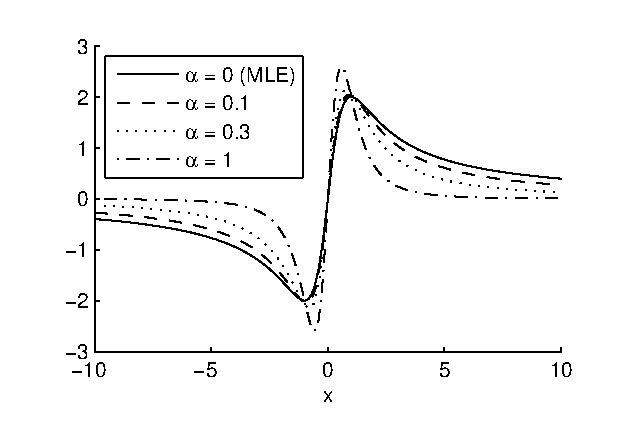
\epsfig{file=Cauchy-IF-mu.eps, height=2.5in} &
	\\	
	& $\mathrm{IF}(x;T_{\mathfrak{R}_\alpha},\mu = 0) $, $\sigma = 1$ is known &
\end{tabular}
\caption{Influence functions of R\'{e}nyi estimator for Cauchy distribution.}
\end{center}
\label{figJK:cauchy-if}
\end{figure}



%%%%%%%%%%%%%%%%%%%%%%%%%%%%% WEIBULL %%%%%%%%%%%%%%%%%%%%%%%%%%%%%%%%%%%%%

\subsection*{Weibull family}
We also succeeded in obtaining some results in the Weibull family with parameters $\theta = (\mu,\lambda, k)$ and probability density
\begin{equation}
	p_\theta =  \frac{k}{\lambda} \left( \frac{x-\mu}{\lambda} \right)^{k-1} \exp \left[ -\left( \frac{x-\mu}{\lambda} \right)^k \right], \qquad \mu>\mathbb{R}, \lambda>0, k>0.
\end{equation}
R\'{e}nyi estimator is given by
\begin{eqnarray}
	\theta_{\alpha,n} & = & \arg \max_{\theta \in \Theta} \left( \frac{k}{\lambda} \right)^\frac{\alpha}{1+\alpha} (1+\alpha)^{\frac{\alpha}{1+\alpha}\frac{1+\alpha+k}{k}} \Gamma\left(\frac{1+\alpha+k}{k}\right)^{-\frac{\alpha}{1+\alpha}} \nonumber \\
						&& \frac{1}{n}\sum_{i=1}^n \left( \frac{x_i-\mu}{\lambda}\right)^{\alpha(k-1)} \exp\left[-\alpha \left(\frac{x_i-\mu}{\lambda}\right)^k\right].
\end{eqnarray}


%%%%%%%%%%%%%%%%%%%%%%%%%%%%%   WEIBULL - IF    %%%%%%%%%%%%%%%%%%%%%%%%%%%%%%%%%%%%%

We will show the resulting influence functions only in figures due to the complexity and length of the formulas. The general shape of the functions is still present. We can see, that the estimator is robust against outliers and that the influence functions are bounded for all $\alpha \neq 0$.

\begin{figure}[!htb]
\begin{center}
\begin{tabular}{cc}
	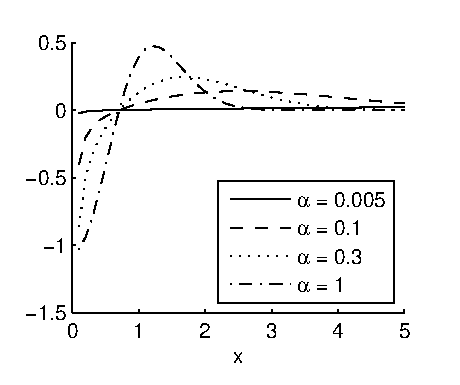
\epsfig{file=Weib-IF-mu.eps, height=2.2in} & 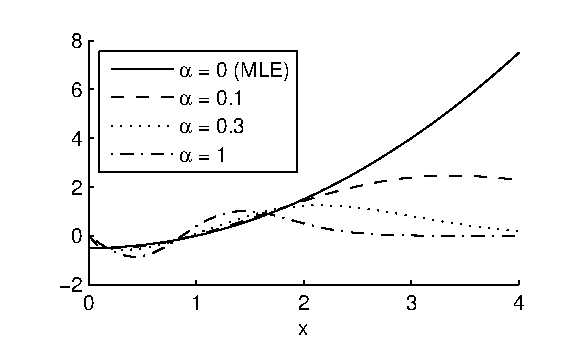
\epsfig{file=Weib-IF-lambda.eps, width=3.2in}
	\\	
	$\mathrm{IF}(x;T_{\mathfrak{R}_\alpha},\mu = 0) $, $\lambda = 1, \: k = 2$ known & $\mathrm{IF}(x;T_{\mathfrak{R}_\alpha},\lambda = 1) $, $\mu = 0, \: k = 2$ are known
\end{tabular}
\caption{Influence functions of R\'{e}nyi estimator for Weibull distribution.}
\end{center}
\label{figJK:weibull-if}
\end{figure}
\begin{figure}[htb]
\begin{center}
\begin{tabular}{cc}	
	\multicolumn{2}{c}{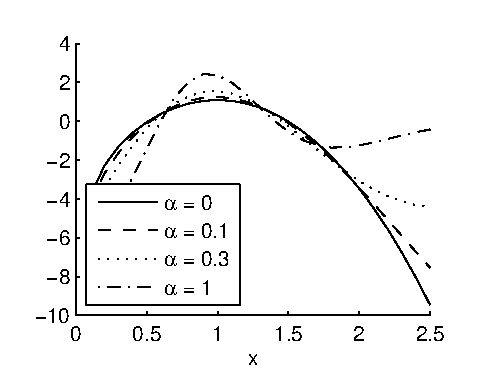
\epsfig{file=Weib-IF-k.eps, height=2.5in}}
	\\
	\multicolumn{2}{c}{$\mathrm{IF}(x;T_{\mathfrak{R}_\alpha},k = 2) $, $\mu = 0, \: \lambda = 1$ are known}
\end{tabular}
\caption{Influence functions of R\'{e}nyi estimator for Weibull distribution.}
\end{center}
\label{figJK:weibull2-if}
\end{figure}

%%%%%%%%%%%%%%%%%%%%%%%%%%%%%   WEIBULL - table    %%%%%%%%%%%%%%%%%%%%%%%%%%%%%%%%%%%%%

\noindent Table \ref{tabJK:weibull-eref} was gained through a different manner than previous ones. We have at disposal the MLE for parameter $\lambda$, but there is none for $\mu$. Because of this, we related the results of estimation of $\mu$ to the estimator with $\alpha = 0.001$. We can see from the table, that the estimates of $\mu$ don't differ significantly with different $\alpha$. On the other hand the estimates of $\lambda$ are much more efficient than MLE. Although Weibull distribution has 3 parameters, we estimated only 2, because our program we used for computing was optimized for minimization of 1- or 2-dimensional distances.

\begin{table}[htb] \footnotesize
\begin{center}
\begin{tabular}{ccc}
	\begin{tabular}{|c|ccc|}
	\hline
	$\alpha\backslash n$ &&  $500$ & \\
	\hline
	& $m(\lambda)$ & $s(\lambda)$ & $eref(\lambda)$ \\
	& $m(\mu)$ & $s(\mu)$ & $eref(\mu)$ \\
	\hline
	$0.0$ & $ 6.462 $ & $ 5.481 $ & $ 1.000 $\\
	$0.001$ & $ -0.006 $ & $ 0.289 $ & $ 1.000 $\\
	\hline
	$0.05$ & $ 1.015 $ & $ 0.289 $ & $ 358.924 $\\
	 & $ 0.005 $ & $ 0.289 $ & $ 0.999 $\\
	\hline
	$0.1$ & $ 1.016 $ & $ 0.284 $ & $ 371.784 $\\
	& $ 0.007 $ & $ 0.282 $ & $ 1.044 $\\
	\hline
	$0.2$ & $ 1.000 $ & $ 0.293 $ & $ 351.092 $\\
	& $ -0.005 $ & $ 0.288 $ & $ 1.004 $\\
	\hline
	$0.3$ & $ 1.010 $ & $ 0.283 $ & $ 376.025 $\\
	 & $ 0.006 $ & $ 0.293 $ & $ 0.968 $\\
	\hline
	$0.5$ & $ 0.998 $ & $ 0.298 $ & $ 337.894 $\\
	 & $ -0.002 $ & $ 0.289 $ & $ 0.998 $\\
	\hline
	$1.0$ & $ 1.005 $ & $ 0.292 $ & $ 352.589 $\\
	 & $ 0.001 $ & $ 0.287 $ & $ 1.012 $\\
	\hline
	\end{tabular}
&&
	\begin{tabular}{c}
		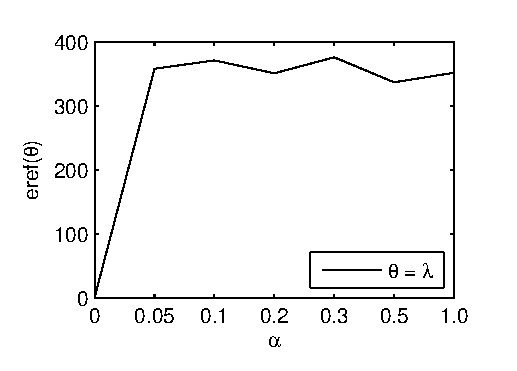
\epsfig{file=Weibull-e04-eref.eps, height=2.5in}
	\end{tabular}
\\
\end{tabular}
\end{center}
\caption{R\'{e}nyi estimates: $p_\theta = \mathrm{W}(0,1,2)$, contamination: $(1-\varepsilon)\mathrm{W}(0,1,2) + \varepsilon \mathrm{W}(0,10,2)$, $\varepsilon =  0.4$.}
\label{tabJK:weibull-eref}
\end{table}


%%%%%%%%%%%%%%%%%%%%%     KONEC   %%%%%%%%%%%%%%%%
\section{Conclusion}
We have studied robust properties of the minimum R\'enyi pseudodistance estimators. We have focused on finding of the corresponding formulas for computing these estimators and their influence functions. We also presented estimation in distributions contaminated with more dispersed observations to present the robustness of R\'enyi estimators against outliers.

\subsection*{Acknowledgment}
This work was supported by the grants SGS12/197/OHK4/3T/14, MSMT INGO-II LG12020, GACR P202/10/0618, and by the research program of the Ministry of Education of Czech Republic under the contract MSM 6840770039.

\begin{thebibliography}{10}

%%examples:
%%Book
%\bibitem{amsbook}
%F. Mittelbach et al.
%\newblock {\em The LaTeX Companion, 2nd ed}.
%\newblock Addison-Wesley, 2004.
%
%%Journal paper
%\bibitem{gned:43}
%B.~V. Gnedenko.
%\newblock Sur la distribution limite du terme maximum d'une s\'{e}rieal\'{e}atoire.
%\newblock {\em Ann. Math.}, {\bf 44}, 423--453, 1943.

\bibitem{Vajda2009}
Michel Broniatowski, Igor Vajda.
\newblock {\em Several Applications of Divergence Criteria in Continuous Families}.
\newblock Research report No 2257 September 2009, UTIA AV CR, Prague, 2009.

\bibitem{Vajda1995}
Igor Vajda.
\newblock {\em Information - Theoretic Methods in Statistics}.
\newblock Research report No 1834 October 1995, UTIA AV CR, Prague, 1995.

\bibitem{Decomposable2011}
Michel Broniatowski, Aida Toma, Igor Vajda.
\newblock {\em Decomposable pseudo-distances and Applications in Statistical Estimation}.
\newblock arXiv:1104.1541v1, 2011.

\bibitem{Demut2010}
Radim Demut.
\newblock {\em Robust properties of minimum divergence density estimators}.
\newblock Diploma Thesis, CTU, Prague 2010.

\bibitem{BasuHarris}
By Ayanendranath Basu, Ian R. Harris, Nils L. Hjort, M. C. Jones.
\newblock {\em Robust and efficient estimation by minimising a density power divergence}.
\newblock In Biometrika, 85, 549-559, 1998.

\bibitem{LieseVajda}
Friedrich Liese, Igor Vajda.
\newblock {\em On Divergences and Informations in Statistics and Information Theory}.
\newblock IEEE Transactions on Information Theory, Vol. 52, No. 10,4394-4412, 2006.


\end{thebibliography}



\end{document}
